\documentclass{article}
\usepackage[preprint]{cs521}
\usepackage{graphicx}
%%%%%% NEED THIS %%%%
\input{epsf.tex}

\title{
Hypergraph Decomposition of Sparse Matrices for Vector-Matrix Multiplication \\[0.3cm]
}
\author{S. Dadizadeh \\[0.1in]
{\em \{sara88\}@cs.ubc.ca} \\
Department of Computer Science \\
University of British Columbia \\
Vancouver, BC, Canada}
\date{Oct 22 2009}

\begin{document}

%%\bibliographystyle{plain}
%%%%%%%%%%%%%%%%%%%%%%%%%%%%%%%%%%%%%%%%%%%
% Start of the Paper 
%%%%%%%%%%%%%%%%%%%%%%%%%%%%%%%%%%%%%%%%%%%

\pagestyle{myheadings}
\thispagestyle{firstheading}

\maketitle
\begin{abstract}

We explore a parallel method of performing sparse matrix multiplication, using hypergraph decomposition to obtain a partitioning of the matrix onto processors. 

\end{abstract}

\vspace{.125in}
\noindent{{\bf Keywords}: hypergraph partitioning, sparse matrix multiplication, matrix-vector multiplication}

\section{Introduction}

Sparse matrix multiplication is one of the most heavily used operations in scientific computing, especially in applications which solve partial differential equations. It is imperative to have scalable matrix operations which perform these computations as efficiently as possible. To achieve the best speed-up possible, we must minimize communication overhead since there are few computations relative to the size of the matrix. Our approach is to model the matrix as a hypergraph and use the MLFM technique to split the hypergraph into partitions, where we assign a partition to each processor \cite{hutchinson}. The problem of finding an optimal partition is NP-hard, but because partitioning is critical in several applications, heursitic algorithms with near-linear runtime were developed \cite{papa}. 

\section{Strategy}

We first need to represent the matrix A as a hypergraph; the model is given in section 2.1. We then use the multilevel Fiduccia-Mattheyses (MLFM) framework to perform the hypergraph partitioning, the algorithm is described in 2.2. In section 3 we delve into implementation details. In 3.1 we give an overview of hMetis, a library that implements the MLFM partitioning algorithm. Finally in 3.2 we describe the implementation details in MPI.

\subsection{Hypergraph Representation}

Our goal is a sparse-matrix vector product of the form \(\vec{y} = A\vec{x}\), where \(\vec{y}\) and \(\vec{x}\) are dense vectors, and \(A\) is a sparse matrix. Matrix \(A\) is represented as the hypergraph \(H_{R}(V_{R}, N_{C})\). The vertex and net sets \(V_{R}\) and \(N_{C}\) correspond to the rows and columns of \(A\), respectively. The vertices in a net \(n_{j}\) are called its pins and denoted as \(pins[n_{j}]\). There exist one vertex \(v _{i}\) and one net \(n_{j}\) for each row \(i\) and column \(j\), respectively. Net \(n_{j}\) contains the vertices corresponding to the columns which have a nonzero entry on row \(j\) (\(v_{i} \in n_{j}\) if and only if \(a_{ij} \neq 0\)). Given this representation, we build a hypergraph \(H\), where the k-way partitioning of \(H\) assigns vertices of \(H\) to \(k\) disjoint nonempty partitions. In a partition \(\Pi\) of \(H\), a net that has at least one pin is said to connect that part. The connectivity set \(\Lambda_{j}\) of a net \(n_{j}\) denotes the number of parts connected by \(n _{j}\). A net \(n _{j}\) is cut if it connects more than one part (\(\Lambda_{j} > 1\)), and uncut otherwise (\(\Lambda_{j} = 1\)). The hypergraph partitioning problem is the task of dividing a hypergraph into two or more parts such that the cutsize is minimized, since cuts represent interprocessor communication.

This decomposition scheme, where we represent rows of A as vertices, and columns of A as hyperedges, is called the column-net model for rowwise decomposition. The nets of \(H_{R}\) represent the dependency relations of the atomic tasks on the \(\vec{x}\)-vector components. Each net \(n_{j}\) incurs the computation \(y_{i} = y_{i} + a_{ij}x_{j}\) for each vertex \(v_{i} \in n_{j}\). This means that each net \(n_{j}\) denotes the set of atomic tasks (vertices) that need \(x_{j}\). Figure 1 illustrates this dependency relation [2]. 

\begin{figure}[htb]
\begin{center}
\mbox{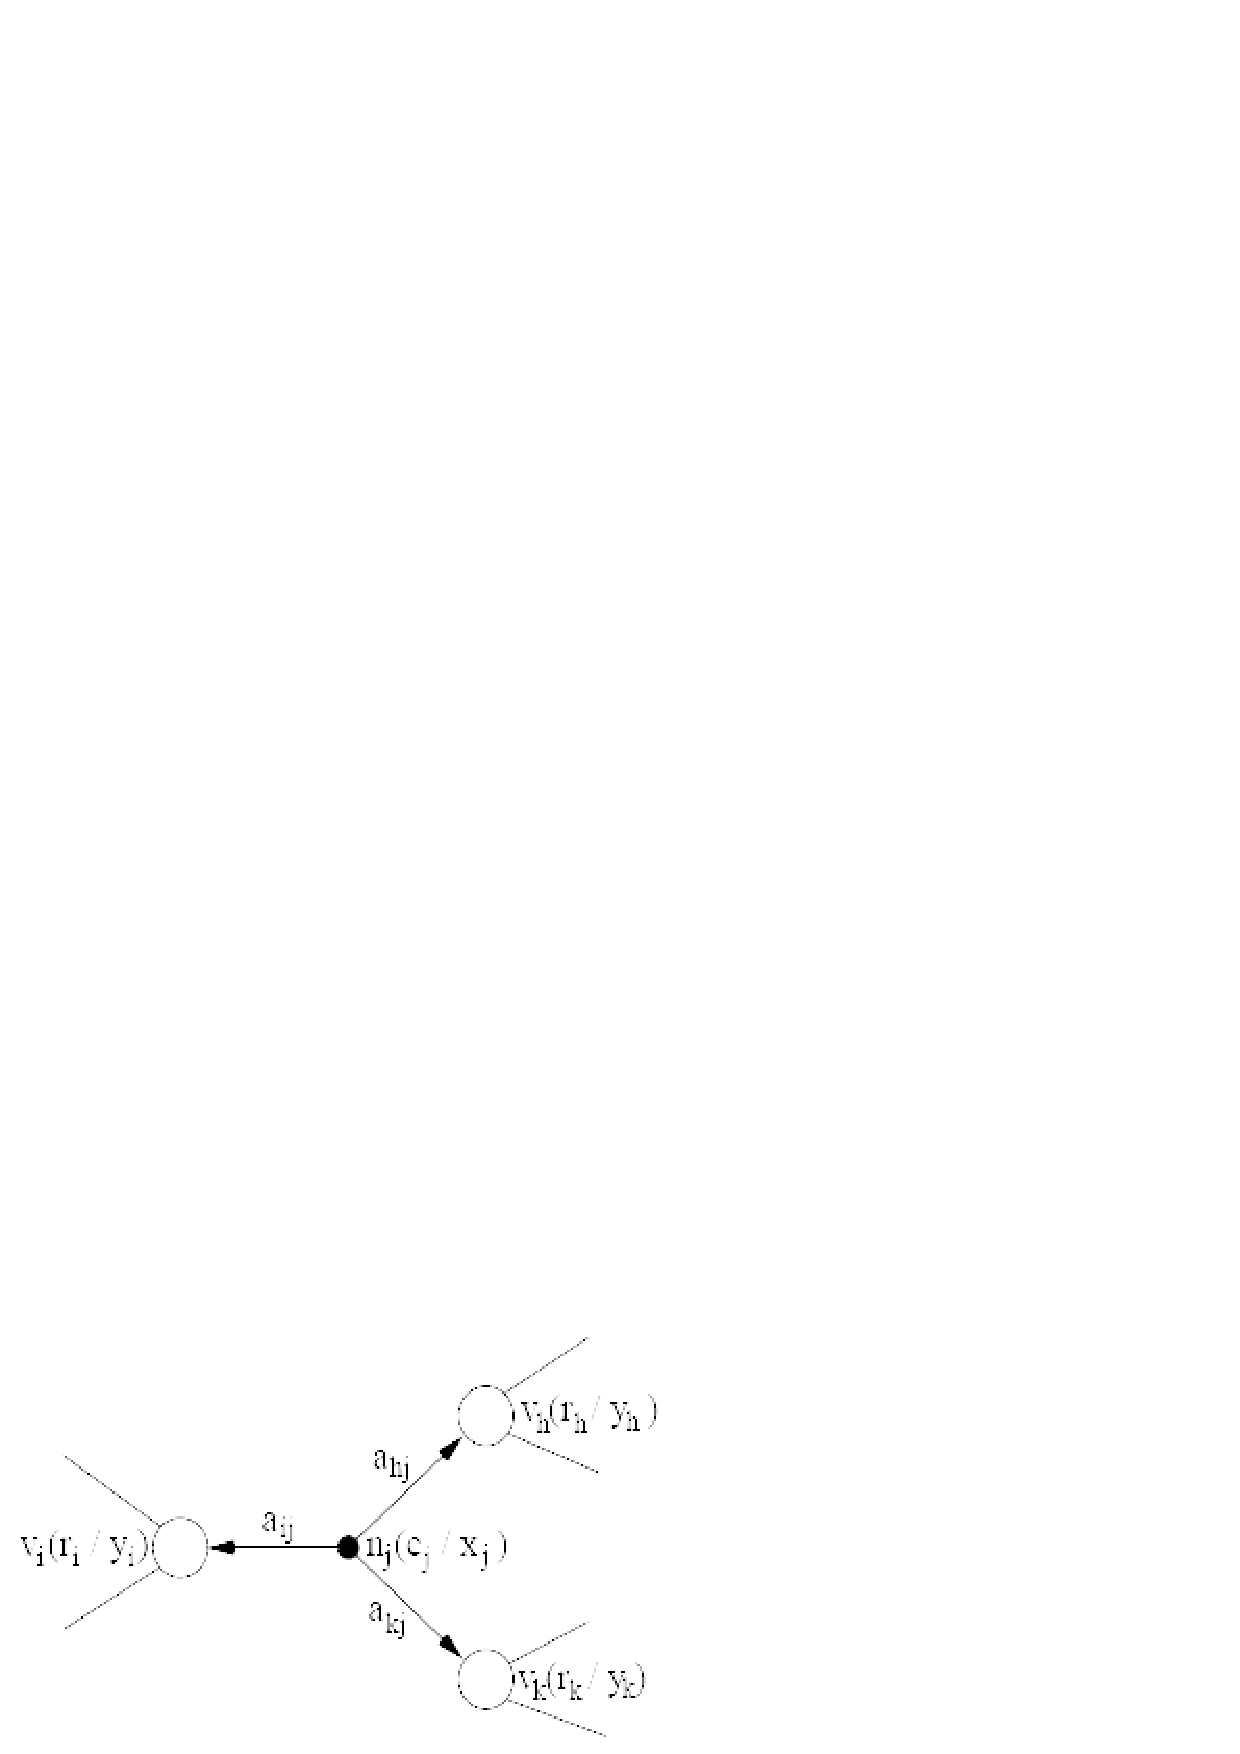
\includegraphics[width=60mm]{columnnet.JPG}}
\end{center}
\caption{Dependency relation view of the column-net model}
\label{fig1}
\end{figure}

\subsection{Hypergraph Partitioning Framework}

The choice of partitioning algorithm depends on the number of movable objects (i.e. the number of vertices). The multilevel Fiduccia-Mattheyses (MLFM) framework scales well with large numbers of vertices, and creates the best known partitioning results. It consists of three components: clustering, top-level partitioning, and refinement or "uncoarsening". During the clustering stage, vertices are combined into clusters based on connectivity, leading to a smaller, clustered hypergraph. Then the smallest (i.e. top-level) hypergraph is partitioned with a fast initial solution generator, and iteratively improved, using the Fidduccia-Mattheyses (FM) partitioning framework (which is a single-level version of the algorithm we use here). During refinement, solutions are projected from one level to the next and iteratively improved, once again by the FM algorithm.

\section{Details of the Implementation}

First we build a hypergraph representation of the matrix A in the format hMetis specifies. We obtain a partitioning from hMetis, and build a structure that contains the data a processor needs to compute its \(y_{i}\) results. Since this data is built dynamically, the root first sends the size, so each process knows how much data to expect. Once the computation is complete, each process sends its \(y_{i}\) results back to the root, where the root aggregates the data to form the result vector \(\vec{y}\).


\begin{figure}[htb]
\begin{center}
\mbox{\includegraphics[width=80mm]{hmetis.JPG}}
\end{center}
\caption{The \texttt{eptr} and \texttt{eind} arrays which describe the hyperedges of the hypergraph.}
\label{fig3}
\end{figure}

\subsection{Overview of hMetis}

hMetis is a hypergraph partitioning package that produces high quality partitions in reasonable time. The main function we are concerned with is \texttt{HMETIS\_PartKway (int nvtxs, int nhedges, int *vwgts, int *eptr, int *eind, int *hewgts, int nparts, int ubfactor, int *options, int *part, int *edgecut)}. \texttt{nvtxs} and \texttt{nhedges} are the number of vertices and hyperedges, respectively. The parameters \texttt{eptr} and \texttt{eind} are two arrays which describe the hyperedges in the graph. \texttt{eptr} is of size \texttt{nhedges}+1, and is used to index into the second array \texttt{eind} that stores the actual hyperedges. Each hyperedge is stored as a sequence of the vertices that it spans, in consecutive locations in \texttt{eind}. \texttt{nparts} is the number of desired partitions. Figure 2 illustrates a simple hypergraph with its corresponding \texttt{eptr} and \texttt{eind} arrays. \texttt{part} returns the computed partition as an array of \texttt{nvtxs} size. Specifically, \texttt{part[i]} contains the partition number in which vertex \(i\) belongs to \cite{hmetis} \cite{cata2}. 

\subsection{Communication and Computation}

In the column-net model, a partition \(\Lambda\) of \(H_{R}\) with \(v_{i} \in P_{k}\) assigns row \(i\), \(y_{i}\) and \(x_{i}\) to processor \(P_{k}\) for rowwise decomposition. A cut net \(n_{j}\) indicates that the processor who contains the corresponding vertex \(v_{j}\) should send its local \(x_{j}\) to all the processors in the connectivity set \(\Lambda _{j}\) of net \(n_{j}\) except itself. For example, in Figure 3, \(P_{1}\) should send \(x_{5}\) to both \(P_{2}\) and \(P_{3}\). Each net \(n_{j}\) incurs the computation \(y_{i} = y_{i} + a_{ij}x_{j}\) for each vertex \(v_{i} \in n_{j}\). Each processor \(P_{k}\) is responsible for computing \(y_{i}\) for the vertices (rows) that it has been assigned.

However, for a processor to know that a net is cut, it must have references to the eptr/eind arrays, as well as the partitioning returned from hMetis. Communicating that much data is infeasible, and the hMetis call is nondeterministic so each processor cannot do the computation locally. Instead, when the root process builds the sparse matrix representation of the data that it needs to distribute to each processor, it appends at the end each \(x_{j}\) value that the corresponding processor will need to perform its computation.

\subsection{Using this Library}

The main function in this library is \texttt{matrix\_multiply(int argc, char** argv, int ubfactor, FILE* matrix\_fp, FILE* vector\_fp, FILE* result\_fp)}. \texttt{argc} and \texttt{argv} are passed from the command line, \texttt{ubfactor} is the unbalance factor, a value ranging from 1 to 49 denoting the amount of unbalance tolerated in the partition (described in \cite{hmetis}). \texttt{matrix\_fp} and \texttt{vector\_fp} are file descriptors, pointing to files which have already been opened for reading. \texttt{result\_fp} is a file descriptor specifying where to write the result vector \(\vec{y}\), and it should already be open for reading. \texttt{finalize()} must be called after \texttt{matrix\_multiply()}, before the program exits.

\begin{figure}[htb]
\begin{center}
\mbox{\includegraphics[width=80mm]{decomp.JPG}}
\end{center}
\caption{A 16x16 sparse matrix A and its column-net representation in a 4-way partitioning}
\label{fig2}
\end{figure}

\section{Performance}

Figure 4 outlines the sequential and parallel run times on varying problem sizes. A matrix size of N denotes a matrix with N*N elements. The parallel version runs much slower than sequential. It is evident that the parallel runtime is dominated by the call to hMetis and the hypergraph creation time. On a problem size of N=10,000, the hMetis call takes 11 seconds, while the sequential version runs in approximately 1 second. Note that the hypergraph creation time can be eliminated by requiring that the matrix be inputted in hypergraph form. 

Since we are employing the column-net model, and need to read the matrix in column-wise, we chose to read the matrix into memory instead of performing many seeks through a large file. This was a poor decision, as very large matrices can be held in memory in sparse matrix format, while there is not enough memory to contain the entire matrix. Because of this issue, there were not enough resources to test this program on large enough matrices where there may have been potential speedup.

\begin{figure}[htb]
\begin{center}
\mbox{\includegraphics[width=85mm]{results.JPG}}
\end{center}
\caption{Benchmarks on a 1.60GHz, 2x Xeon duo core with 8GB memory. All timing values are in seconds.}
\label{results}
\end{figure}

\section{Conclusions}

Although this implementation did not yield desirable results, hypergraph decomposition has been shown to find partitions which deliver significantly better performance than simply distributing sets of rows or columns onto processors. Given a few adjustments to the design and implementation of this program, we are confident that this method will result in a high performance sparse matrix multiplier.

\bibliographystyle{unsrt}
\bibliography{mybib}

\end{document}
